\lab{PCA, LSI, and Scikit-Learn}{LSI and SkLearn}
\objective{Understand the basics of principal component analysis and latent semantic indexing. Learn more about scikit-learn and implement a machine learning pipeline.}
\label{lab:pca} 

\section*{Principal Component Analysis} % --------------------------------------------------

Principal Component Analysis (PCA) is a multivariate statistical tool used to change the basis of a set of samples from the basis of original features (which may be correlated) into a basis of uncorrelated variables called the \emph{principal components}.
It is a direct application of the singular value decomposition (SVD).
The first principal component will account for the greatest variance in the samples, the second principal component will be orthogonal to the first and account for the second greatest variance, etc.
By projecting the samples onto the space spanned by the first few principal components, we can reduce the dimensionality of the data while preserving most of the variance.

Take a matrix $X$ with samples as rows and features as columns.
The first step in PCA is to pre-process the data, which usually includes translating the columns of $X$ to have mean 0.
Some datasets require additional scaling based on variance and units of measurement.
Call the new pre-processed matrix $Y$.

We next compute the truncated SVD of our centered data, $Y = U\Sigma V^{T}$, where the columns of $V$ are the principal components and form an orthonormal basis for the space spanned by the samples.
The variance captured by each principal component can be calculated by the equation below, where $\sigma_{i}$ is the $i$-th nonzero singular value and there are $k$ total singular values.
\begin{equation}
\frac{\sigma^2_{i}}{\sum_{j=1}^{k} \sigma^2_{j}}
\label{equation:pc}
\end{equation}

In general, we are only interested in the first several principal components.
But just how many principal components should we keep?
One method is to keep the first two principal components so that we can project the data into $2$-dimensional space.
Another is to only keep the set of principal components accounting for a certain percentage of the variance, using the equation above.

Once we have decided how many principal components to keep (say the first $l$), we can project the samples from the original feature space onto the principal component space by computing
\begin{equation*}
\widehat{Y} = U_{:,:l}\Sigma_{:l,:l} = YV_{:,:l}
\end{equation*}

\begin{problem}% Problem 1

The breast cancer dataset from scikit-learn has 569 samples with 30 features each.
Each sample is labeled as \li0 (malignant) or \li1 (benign).
With 30 features, this data can't be directly visualized, so we will use PCA to graph the first two principal components, which account for nearly all of the variance in the data.

Write a function that performs PCA on the breast cancer dataset using the SVD as described above.
Graph the first two principal components, with the first along the $x$-axis.
Your graph should resemble Figure \ref{fig:cancer} below.
Include the proportion of the total variance that the first two principal components capture in the graph title, calculated with Equation \ref{equation:pc}.
\label{problem:cancer}

You can load this dataset using the following code:
\begin{lstlisting}
>>> cancer = sklearn.datasets.load_breast_cancer()
>>> X = cancer.data
>>> y = cancer.target # Class labels (0 or 1)
\end{lstlisting}
\end{problem}

\begin{figure}[H]
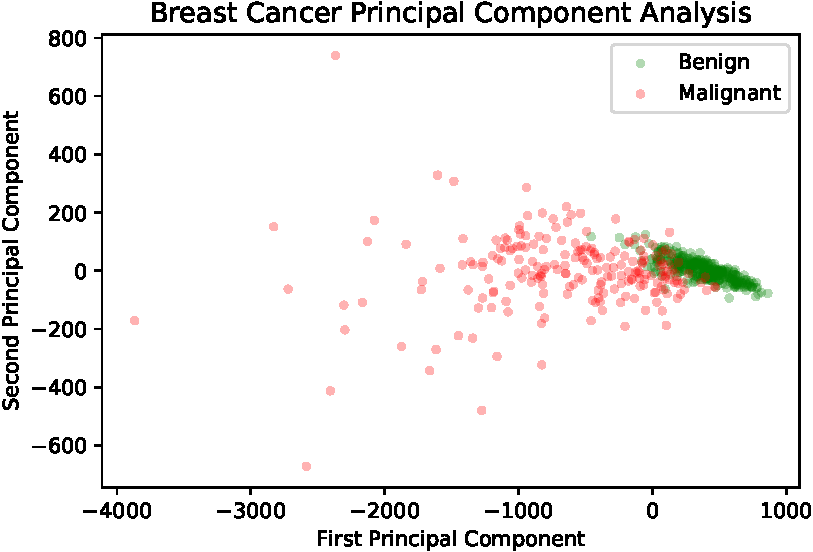
\includegraphics[width=.7\textwidth]{figures/cancer.pdf}
\caption{First two principal components of the transformed breast cancer data}
\label{fig:cancer}
\end{figure}

\section*{Latent Semantic Indexing} % --------------------------------------------------

\emph{Latent Semantic Indexing} (LSI) is an application of PCA to the realm of natural language processing.
In particular, LSI employs the SVD to reduce the dimensionality of a large corpus of text documents in order to enable us to evaluate the similarity between two documents.
Many information-retrieval systems used in government and in industry are based on LSI.

To motivate the problem, suppose we have a large collection of documents about various topics.
How can we find an article about BYU? %Would like to find a better example here.
We might consider simply choosing the article that contains the acronym the greatest number of times, but this is a crude method.
A better way is to use a form of PCA on the collection of documents.

In order to do so, we need to represent the documents as numerical vectors.
A standard way of doing this is to define an ordered set of words occurring in the collection of documents (called the \emph{vocabulary}) and then to represent each document as a vector of word counts from the vocabulary.
More formally, let our vocabulary be $V = \{w_1,w_2,\ldots,w_m\}$.
Then a document is a vector $x  = (x_1,x_2,\ldots,x_m) \in \mathbb{R}^m$ such that $x_i$ is the number of occurrences of word $w_i$ in the document.
In this setup, we represent the entire collection of $m$ documents as an $n \times m$ matrix $X$, where $m$ is the number of vocabulary words and $n$ is the number of documents in our collection, so each row is a document vector.
As expected, we let $X_{i,j}$ be the number of times term $j$ occurs in document $i$.
Note that $X$ is often a sparse matrix, as any single document likely does not contain most of the vocabulary words.
This mode of representation is called the \emph{bag of words} model for documents.

We calculate the SVD of $X$ \emph{without} centering or scaling the data so that we may retain the sparsity. 
This is unique to this particular problem.
We now have $X = U\Sigma V^T$.
If we are keeping $l$ principal components, we can represent the corpus of documents by the matrix
\[
\widehat{X} = U_{:,:l}\Sigma_{:l,:l} = XV_{:,:l}
\]
Note that $\widehat{X}$ will no longer be a sparse matrix, but will have dimension $n \times l$.

Now that we have our documents represented in terms of the first $l$ principal components, we can find the similarity between two documents.
Our measure for similarity is simply the cosine of the angle between the vectors; a small angle (large cosine) indicates greater similarity, while a large angle (small cosine) indicates greater dissimilarity.
Recall that we can use the inner product to find the cosine of the angle between two vectors.
Under this metric, the similarity between document $i$ and document $j$ (represented by the $i$-th and $j$-th row of $\widehat{X}$, notated $\widehat{X}_i$ and $\widehat{X}_j$, respectively) is just
\[
\frac{\langle \widehat{X}_i, \widehat{X}_j\rangle}{\|\widehat{X}_i\|\|\widehat{X}_j\|}.
\]
To find the document most similar to document $i$, we simply compute
\[
\argmax_{j\neq i} \frac{\langle \widehat{X}_i, \widehat{X}_j\rangle}{\|\widehat{X}_i\|\|\widehat{X}_j\|}.
\]

\begin{problem} %Problem 2
Create a function \li{similar} that takes in a numpy array \li{Xhat} and an index \li{i} and returns the indices of the most similar and the least similar documents.

Hint: \li{np.argsort} may be useful for finding which are the most and least similar.
Note that every document will have a similarity score of 1 with itself, so be careful not to return a document as its own closest document.

To test your code, use the following matrix:
\begin{lstlisting}
X = np.array([
    [0.78, 0.14, 0.12, 0.  ],
    [0.64, 0.97, 0.  , 0.  ],
    [0.  , 0.  , 0.63, 0.46],
    [0.  , 0.84, 0.6 , 0.  ],
    [0.29, 0.89, 0.51, 0.  ],
    [0.77, 0.  , 0.27, 0.2 ],
    [0.86, 0.47, 0.  , 0.06],
    [0.89, 0.  , 0.  , 0.  ]
]) 
\end{lstlisting}
With \li{i=4} your function should output the following:
\begin{lstlisting}
>>> print(similar(4, X))
(7, 3)
\end{lstlisting}
\end{problem}

\section*{Application: State of the Union} 
We now discuss some practical issues involved in creating the bag of words representation $X$ from the raw text.
Our dataset will consist of the US State of the Union addresses from 1945 through 2013, each contained in a separate text file in the folder {\tt Addresses}.
We would like to avoid loading in all of the text into memory at once, and so we will \emph{stream} the documents one at a time.

The first thing we need to establish is the vocabulary set, i.e. the set of unique words that occur throughout the collection of documents.
A Python set object automatically preserves the uniqueness of the elements, so we will create a set and then iteratively read through the documents, adding the unique words of each document to the set.
As we read in each document, we will remove punctuation and numerical characters and convert everything to lower case.
The following code, found in the function \li{document_converter()}, will accomplish this task. 

\begin{lstlisting}
# Get list of filepaths to each text file in the folder.
folder = "./Addresses/"
paths = sorted([folder+p for p in os.listdir(folder) if p.endswith(".txt")])

# Helper function to get list of words in a string.
def extractWords(text):
    ignore = string.punctuation + string.digits
    cleaned = "".join([t for t in text.strip() if t not in ignore])
    return cleaned.lower().split()

# Initialize vocab set, then read each file and add to the vocab set.
vocab = set()
for p in paths:
    with open(p, 'r', encoding="utf8") as infile:
        for line in infile:
            vocab.update(extractWords(line)) # Union sets together
\end{lstlisting}

We now have a set containing all of the unique words in the corpus.
However, many of the most common words do not provide important information.
We call these \emph{stop words}. Examples in English include \emph{the, a, an, and, I, we, you, it, there}, etc; a list of common English stop words is given in \texttt{stopwords.txt}.
We remove the stop words from our vocabulary set as follows and then fix an ordering to the vocabulary by creating a dictionary
with key-value pairs of the form (word, index).

\begin{lstlisting}
# Load stopwords
with open("stopwords.txt", 'r',  encoding="utf8") as f:
    stops = set([w.strip().lower() for w in f.readlines()])

# Remove stopwords from vocabulary, create ordering
vocab = {w:i for i, w in enumerate(vocab.difference(stops))}
\end{lstlisting}

We are now ready to create the word count vectors for each document, and we store these in a sparse matrix $X$.
It is convenient to use the \li{Counter} object from the \li{collections} module, as this object automatically counts the occurrences of each distinct element in a list.

\begin{lstlisting}
from collections import Counter

counts = []      # holds the entries of X
doc_index = []   # holds the row index of X
word_index = []  # holds the column index of X

# Iterate through the documents
for doc, p in enumerate(paths):
    with open(p, 'r', encoding="utf8") as f:
        # Create the word counter.
        ctr = Counter()
        for line in f:
            ctr.update(extractWords(line))
        # Iterate through the word counter, storing counts.
        for word, count in ctr.items():
            if word in vocab:
                word_index.append(vocab[word])
                counts.append(count)
                doc_index.append(doc)

# Create sparse matrix holding these word counts.
X = sparse.csr_array((counts, [doc_index, word_index]),
                       shape=(len(paths), len(vocab)), dtype=float)
\end{lstlisting}

\begin{problem} %Problem 3
Applying the techniques of LSI discussed above to the word count matrix $X$, created with the \li{document_converter()} function, and keeping the first 7 principal components, write a function that takes in the path to a single State of the Union address \li{speech} and returns a tuple of the addresses that are most and least similar to \li{speech}.

For Ronald Reagan's 1984 speech, the input would be \li{'./Addresses/1984-Reagan.txt'}, and your output should be \li{('1985-Reagan', '1946-Truman')}.
Be sure to format the strings properly. 
Also run your algorithm on Clinton's 1993 speech, and display your output.

Since $X$ is a sparse matrix, you will need to use the SVD method found in \li{scipy.sparse.linalg}.
This method operates slightly differently than the SVD method found in \li{scipy.linalg}, so be sure to read the documentation.
Also pass the argument \li{random_state=28} into this function for consistency.
\label{prob:LSI1}
\end{problem}

The simple bag of words representation is a bit crude, as it fails to consider how some words may be more important than others in determining the similarity of documents.
Words appearing in few documents tend to provide more information than words occurring in every document.
For example, while the word \emph{war} might not be considered a stop word, it is likely to appear in many more addresses than the word \emph{Afghanistan}.
Two speeches sharing the word \emph{Afghanistan} are probably more closely related than two speeches sharing the word \emph{war}.
So while $X_{i,j}$ is a good measure of the importance of term $j$ in document $i$, we also need to consider some kind of global weight for each term $j$, indicating how important the term is over the entire collection.
There are a number of different weights we could choose; we will employ the following approach.
Define
\begin{equation*}
p_{i,j} = \frac{X_{i,j}}{\sum_{\bar{\jmath}} X_{i,\bar{\jmath}}}.
\end{equation*}
We then let
\begin{equation*}
g_{j} = 1 + \sum_{i=1}^{m} \frac{p_{i,j} \log (p_{i,j} + 1)}{\log m},
\end{equation*}
where $m$ is the number of documents in the collection.
We call $g_{j}$ the \emph{global weight} of term $j$.
We replace each term frequency in the matrix $X$ by weighting it globally.
Specifically, we define a matrix $A$ with entries
\begin{equation*}
A_{i,j} = g_{j} \log (X_{i,j} + 1).
\end{equation*}
We can now perform LSI on the matrix $A$, whose entries are both locally and globally weighted.

\begin{problem} %Problem 4
Use the equation above to create the function \li{weighted_document_converter()} to calculate the sparse matrix $A$.
Similar to the function \li{document_converter()}, this function should return $A$ and a list of file paths.

Hint: the function \li{np.log1p}, which calculates $\log(1+x)$, can be applied to a sparse matrix without losing sparsity.
\label{problem:global-weights}
\end{problem}

\section*{Scikit-Learn} % --------------------------------------------------

Scikit-learn is one of the fundamental tools Python offers for machine learning.
It includes classifiers, such as \li{RandomForestClassifier} and \li{KNeighborsClassifier}, as well as transformers, which preprocess data before classification.
In the remainder of this lab, we will discuss transformers, validation tools, how to find optimal hyperparameters, and how to build a machine learning pipeline.

\subsection*{Transformers} % --------------------------------------------------

A scikit-learn \emph{transformer} processes data to make it better suited for classification.
This may involve shifting or scaling data, dropping columns, replacing missing values, and so on.
The function from Problem \ref{problem:global-weights} is an example of a transformer, as is PCA.

\begin{info}
A \emph{hyperparameter} is not dependent on data.
Hyperparameters are declared in the constructor \li{__init__()}, before data is even passed in.
Parameters set during the \li{fit()} method are often called \emph{model parameters} and do depend on specific data.
For example, a \li{StandardScaler} transformer shifts and scales data to have a mean of 0 and a standard deviation of 1.

Scikit-learn's transformers have three main methods: \li{fit_transform()}, which fits model parameters and also transforms given data; \li{fit()}, which sets model parameters but does not perform a transformation; and \li{transform()}, which transforms data according to pre-fitted model parameters.
Model parameters are fitted according to training data, and they are not refitted to testing data, so a \li{StandardScaler} will shift and scale testing data according to the mean and variance of the training data; the transformed test data likely will not have mean 0 and variance 1.
\end{info}

Scikit-learn has a built-in PCA package.
Its hyperparameters include the desired number of principal components and the type of SVD solver to use.
Its \li{fit_transform()} method takes in an array of data and returns the decomposition with \li{n_components}.

\begin{lstlisting}
>>> from sklearn.decomposition import PCA 
>>> pca = PCA(n_components=5) # Create the PCA transformer with hyperparameters
>>> Xhat = pca.fit_transform(X) # Fit the transformer and transform the data
\end{lstlisting}

For our particular application, however, ince our matrix is sparse and Scikit-learn's \li{PCA} class does not accept sparse matrices, we need to use their \li{TruncatedSVD} class instead.
The syntax for this class is identical to the above.

\begin{info}
An interesting observation can be made by repeating Problem \ref{problem:cancer} using scikit-learn's PCA package.
The resulting graph will have the $x$-axis flipped, because a matrix's singular value decomposition is unique up to multiplication by -1.
\end{info}

\begin{problem} %Problem 5
Repeat Problem \ref{prob:LSI1} using your weighted document converter function and scikit-learn's \li{sklearn.decomposition.TruncatedSVD} class.
For consistency, also pass the argument \li{random_state=74} in the constructor to this class.

For Bill Clinton's 1993 speech, your code should return \li{('1994-Clinton', '1946-Truman')}.
Also run the algorithm on Reagan's 1984 speech, and display the results.
\end{problem}

\subsection*{Validation Tools} % ----------------------------------------------------

We now turn our attention from transformers to classifiers.
A \emph{classifier} is trained to predict how a new sample should be classified or labeled.
Knowing how to determine whether or not a classifier performs well is an essential part of machine learning.
This often turns out to be a surprisingly sophisticated issue that largely depends on the type of problem being solved and the kind of data that is available for training.
Scikit-learn has validation tools for many situations; for brevity, we restrict our attention to the simple (but important) case of \emph{binary classification}, where the possible labels are only \li0 or \li1.

The \li{score()} method of a scikit-learn classifier returns the \emph{accuracy} of the model, or the percent of labels predicted correctly.
However, accuracy isn't always the best measure of success.
Consider the \emph{confusion matrix} for a classifier, the matrix where the $(i,j)$th entry is the number of samples with actual label $i$ but that are classified with label $j$.
Call the class with label $0$ the \emph{negatives} and the class with label $1$ the \emph{positives}.
Then the confusion matrix is as follows. 

\begin{align*}
\begin{blockarray}{ccc}
& \textrm{Predicted: }0 & \textrm{Predicted: }1 \\
\begin{block}{c[cc]}
\textrm{Actual: }0 & \textrm{True Negatives } (TN) & \textrm{False Positives } (FP)\\
\textrm{Actual: }1 & \textrm{False Negatives } (FN) & \textrm{True Positives } (TP)\\
\end{block}\end{blockarray}
\end{align*}

With this terminology, we define the following metrics.
\begin{itemize}
\item \emph{Accuracy}: $\dfrac{TN + TP}{TN + FN + FP + TP}$, the percent of labels predicted correctly.
\item \emph{Precision}: $\dfrac{TP}{TP + FP}$, the percent of predicted positives that are actually correct. %How many selected items were relevant
\item \emph{Recall}: $\dfrac{TP}{TP + FN}$, the percent of actual positives that are predicted correctly. %How many relevant items were selected
\end{itemize}

Precision is useful in situations where false positives are dangerous or costly, while recall is important when avoiding false negatives takes priority.
For example, an email spam filter should avoid filtering out an email that isn't actually spam; here a false positive is more dangerous, so precision is a valuable metric for the filter.
On the other hand, recall is more important in disease detection: it is better to test positive and not have the disease than to test negative when the disease is actually present.
Focusing on a single metric often leads to skewed results, so the following metric is also common.

\begin{equation*}
F_\beta \text{ Score}: (1 + \beta^2)
\dfrac{\text{precision}\cdot\text{recall}}{(\beta^2\cdot\text{precision}) + \text{recall}} = \dfrac{(1 + \beta^2)TP}{(1+\beta^2)TP + FP + \beta^2 FN}.
\end{equation*}

Choosing $\beta < 1$ weighs precision more than recall, while $\beta > 1$ prioritizes recall over precision.
The choice of $\beta = 1$ yields the common $F_1$ score, which weighs precision and recall equally.
This is an important alternative to accuracy when, for example, the training set is heavily unbalanced with respect to the class labels.

Scikit-learn implements all of these metrics in \li{sklearn.metrics}.
The general syntax for such functions is \li{some_score(actual_labels, predicted_labels)}.
We will be using the function \li{classification_report()}, which returns precision, recall, and $F_1$ scores for each label.
Each row in the report corresponds to a specific label and gives the scores with its label as the "positive" classification.
For example, in binary classification, the row corresponding to \li1 gives the scores as they would normally be calculated, with \li1 as "positive."

\begin{lstlisting}
>>> from sklearn.neighbors import KNeighborsClassifier
>>> from sklearn.metrics import confusion_matrix, classification_report
>>> from sklearn.model_selection import train_test_split

# Split the data into training and testing sets
>>> X_train, X_test, y_train, y_test = train_test_split(X, y)

# Fit the esimator to training data and predict the test labels.
>>> knn = KNeighborsClassifier(n_neighbors=2)
>>> knn.fit(X_train, y_train)
>>> knn_predicted = knn.predict(X_test)

# Compute the confusion matrix by comparing actual labels to predicted labels.
>>> CM = confusion_matrix(y_test, knn_predicted)
>>> CM
array([[44,  5],
       [10, 84]])

# Get precision, recall, and F1 scores all at once.
# The row labeled 1 gives these scores as we normally calculate them.
>>> print(classification_report(y_test, knn_predicted))
<<              precision    recall  f1-score   support

           0       0.81      0.90      0.85        49
           1       0.94      0.89      0.92        94

    accuracy                           0.90       143
   macro avg       0.88      0.90      0.89       143
weighted avg       0.90      0.90      0.90       143>>
\end{lstlisting}

\begin{problem} %Problem 6
For this problem, use the cancer dataset from Problem \ref{problem:cancer} to compare a \\ \li{RandomForestClassifier} and a \li{KNeighborsClassifier}, using the default parameters for each.

Use \li{train_test_split()} with \li{random_state=2} to split up the data.
Fit the classifiers with the training set and predict the labels for the testing set.
Print out a classification report for each classifier, making sure to clearly label which report corresponds to which classifier.

Write a few sentences explaining which of these classifiers would be better to use in this situation and why, using the information from the report as evidence.
Remember that in this dataset, the label \li1 means benign and \li0 means malignant.
\label{problem:validation}
\end{problem}

\subsection*{Grid Search} % ---------------------------------------------------

Finding the optimal hyperparameters for a given model is a challenging and active area of research.\footnote{Intelligent hyperparameter selection is sometimes called \emph{metalearning}.}
However, brute-force searching over a small hyperparameter space is simple in scikit-learn: a \li{sklearn.model_selection.GridSearchCV} object is initialized with a classifier, a dictionary of hyperparameters, and some validation parameters.
When its \li{fit()} method is called, it tests the given classifier with every possible hyperparameter combination.

For example, a \li{KNeighborsClassifier} has a few important hyperparameters that can have a significant impact on the speed and accuracy of the model.
These include \li{n_neighbors}, the number of nearest neighbors allowed to vote, and \li{weights}, which specifies a strategy for weighting the distances between points.
The code box below tests various combinations of these hyperparameters.

The cost of a grid search rapidly increases as the hyperparameter space grows.
However, the outcomes of each trial are completely independent of each other, so the problem of training each classifier is \emph{embarassingly parallel}, meaning the trials can easily be computed simultaneously.
To parallelize the grid search over $n$ CPU cores, set the \li{n_jobs} parameter to $n$, or set it to $-1$ to divide the labor between as many cores as are available.

\begin{lstlisting} 
>>> from sklearn.model_selection import GridSearchCV

>>> knn = KNeighborsClassifier()
# Specify values for certain hyperparameters
>>> param_grid = {"n_neighbors": [2, 3, 4, 5, 6],
...               "weights": ["uniform", "distance"]}
>>> knn_gs = GridSearchCV(knn, param_grid, scoring="f1", n_jobs=-1)

# Run the actual search. This may take some time.
>>> knn_gs.fit(X_train, y_train)

# After fitting, you can access data about the results.
>>> print(knn_gs.best_params_, knn_gs.best_score_, sep='\n')
<<{'n_neighbors': 5, 'weights': 'uniform'}
0.9532526583188765>>

# Access the model
>>> knn_gs.best_estimator_
KNeighborsClassifier(weights='distance')
\end{lstlisting}

In some circumstances, the parameter grid can be organized in a way that eliminates redundancy.
For example, with a \li{RandomForestClassifier}, you could test each \li{max_depth} argument with entirely different sets of values for \li{min_samples_leaf}.
To specify certain combinations of parameters, enter the parameter grid as a list of dictionaries.

\begin{problem} %Problem 7
Do a grid search on the breast cancer dataset using a \li{RandomForestClassifier}.
Modify at least three parameters in your grid.
Use  \li{scoring="f1"} for the \li{GridSearchCV} object.
Fit your model with the same train-test split as in Problem \ref{problem:validation}.
Print out the best parameters and the best score.

Next, use the \li{GridSearchCV} object to predict labels for your test set.
Print out a confusion matrix using these values.
\label{problem:gridsearch}
\end{problem}

\section*{Pipelines} % ========================================================

Most machine learning problems require at least a little data preprocessing before estimation in order to get good results.
A scikit-learn \emph{pipeline} chains together one or more transformers and one estimator (such as a classifier) into a single object, complete with \li{fit()} and \li{predict()} methods.
This simplifies and automates the machine learning process so that when you get new data or make changes to various functions and features, you can easily rerun the new version from beginning to end.

The following example demonstrates how to use a pipeline with a \li{StandardScaler} transformer and a \li{KNeighborsClassifier}.
Like classifiers, pipelines have \li{fit()}, \li{predict()}, and \li{score()} methods.
Each member of the pipeline is declared as a tuple where the first element is a string naming the step and the second is the actual transformer or classifier.

\begin{lstlisting}
>>> from sklearn.preprocessing import StandardScaler
>>> from sklearn.pipeline import Pipeline

# Chain together a StandardScaler transformer and a KNN classifier.
>>> pipe = Pipeline([("scaler", StandardScaler()), # "scaler" is the step name
...                  ("knn", KNeighborsClassifier())]) # "knn" is the step name
>>> pipe.fit(X_train, y_train)
>>> pipe.score(X_test, y_test)
0.972027972027972
\end{lstlisting}

Since \li{Pipeline} objects follow \li{fit()} and \li{predict()} conventions, they can be used with tools like \li{GridSearchCV}.
To specify which hyperparameters belong to which steps of the pipeline, precede each hyperparameter name with \li{<stepname>__}.
For example, \li{knn__n_neighbors} corresponds to the \li{n_neighbors} hyperparameter of the pipeline step labeled \li{knn}.

\begin{lstlisting}
# Create the Pipeline, labeling each step.
>>> pipe = Pipeline([("scaler", StandardScaler()),
                     ("knn", KNeighborsClassifier())])
                     
# Specify the hyperparameters to test for each step.
>>> pipe_param_grid = {"scaler__with_mean": [True, False],
...                    "scaler__with_std": [True, False],
...                    "knn__n_neighbors": [2,3,4,5,6],
...                    "knn__weights": ["uniform", "distance"]}

# Pass the Pipeline object to the GridSearchCV and fit it to the data.
>>> pipe_gs = GridSearchCV(pipe, pipe_param_grid,
...                        n_jobs=-1).fit(X_train, y_train)

>>> print(pipe_gs.best_params_, pipe_gs.best_score_, sep='\n')
<<{'knn__n_neighbors': 6, 'knn__weights': 'distance',
 'scaler__with_mean': True, 'scaler__with_std': True}
0.971830985915493>>
\end{lstlisting}

Pipelines can also be used to compare different transformations or estimators.
For example, a pipeline can end in either a \li{KNeighborsClassifier()} or a classifier called \li{SVC()}, even though they have different hyperparameters.
Like before, you can use a list of dictionaries to specify the specific combinations of the hyperparameter space.

\begin{lstlisting}
# Create the pipeline, using any classifier as a placeholder
>>> pipe = Pipeline([("scaler", StandardScaler()),
                     ("classifier", KNeighborsClassifier())])

# Create the grid
>>> pipe_param_grid = [
...     {"classifier": [KNeighborsClassifier()],    # Try a KNN classifier...
...      "classifier__n_neighbors": [2,3,4,5],
...      "classifier__weights": ["uniform", "distance"]},
...     {"classifier": [SVC(kernel="rbf")],         # ...and an SVM classifier.
...      "classifier__C": [.001, .01, .1, 1, 10, 100],
...      "classifier__gamma": [.001, .01, .1, 1, 10, 100]}]

# Fit using training data
>>> pipe_gs = GridSearchCV(pipe, pipe_param_grid,
...                        scoring="f1", n_jobs=-1).fit(X_train, y_train)

# Get the best hyperparameters
>>> params = pipe_gs.best_params_
>>> print("Best classifier:", params["classifier"])
<<Best classifier: SVC(C=10, cache_size=200, class_weight=None, coef0=0.0,
  decision_function_shape='ovr', degree=3, gamma=0.01, kernel='rbf',
  max_iter=-1, probability=False, random_state=None, shrinking=True,
  tol=0.001, verbose=False)>>

# Check the best classifier against the test data
>>> confusion_matrix(y_test, pipe_gs.predict(X_test))
array([[48,  1],                        # Near perfect!
       [ 1, 93]])
\end{lstlisting}

\begin{problem} %Problem 8
The breast cancer dataset has 30 features.
By using PCA, we can drastically reduce the dimensionality while still retaining predictive power.

Create a pipeline with a \li{StandardScaler}, \li{PCA}, and a \li{KNeighborsClassifier}.
Use the same train-test split as before.
Do a grid search on this pipeline, modifying at least six hyperparameters and using \li{scoring="f1"}.
Use no more than 5 principal components.
Print out your best parameters and best score.
Attain a score of at least .96.

\emph{Hint:} The documentation for \href{https://scikit-learn.org/stable/modules/generated/sklearn.preprocessing.StandardScaler.html}{\li{StandardScaler}}, \href{https://scikit-learn.org/stable/modules/generated/sklearn.decomposition.PCA.html}{\li{PCA}}, and \href{https://scikit-learn.org/stable/modules/generated/sklearn.neighbors.KNeighborsClassifier.html}{\li{KNeighborsClassifier}} can be found at these links.
\end{problem}





